\chapter{Vizualizace dat}
\label{ch:vizualizace}

Očištěná data zaznamenaných shrinků vybrané společnosti jsem vizualizovala v nástroji Power BI, který se používá pro business intelligence anlýzu. Vytvořila jsem report, který umožňuje pomocí interaktivních grafů analyzovat data. První část této kapitoly se věnuje technickému popisu reportu, zatímco druhá část shrnuje výsledky analýzy plynoucí z reportu.

\section{Popis řešení}
\label{sec:vizualizace:popis}

Report obsahuje pět stránek. První stránka nabízí základní přehled, dashboard, týkající se všech shrinků. Druhý list je věnován prodejnám a údajům o lokalitách.
Další stránky se již věnují pouze shrinkům zaviněných škodami a kategoriím Velmi čerstvé a Čerstvé z produktové hiearchie úrovně 1. Třetí list zobrazuje hodnoty ukazatelů hodnoty shirnku a odvozených podílů. Na čtvrtém a pátem listu jsou další přehledy z pohledu konkrétních produktů, kategorií a typů promoakce. Poslední stránka týkající se reportingu je z pohledu vybraného konkrétního produktu.

Do Power BI souboru jsem pomocí integrovaného nástroje PowerQuery nahrála upravená data z databáze vybrané společnosti. Hlavní faktickou tabulkou je tabulka \emph{damages}, která obsahuje všechny zaznamenané shrinky z kategorie shrinků, které byly způsobeny škodami. Druhá faktická tabulka má název \emph{revenue} a obsahuje tržby v pozorovaném měsíci pro všechny prodejny, tržby jsou dále rozdělené podle kategorie z úrovně 1 a do čtvrtin měsíce. Doménové tabulky jsou číselník produktů, číselník shrinků a číselník prodejen, dále také číselníkové tabulky, které spojují faktické tabulky -- čtvrtina měsíce a seznam kategorií úrovně 1. 

Datový model tabulek, které jsou vstupem do reportu je znázorněný na obrázku \ref{obr:datmod}. Mezi jednotlivými tabulkami jsou znázorněny vazby -- jejich mohutnost a směr. Tabulka \emph{metrics}, která není navázaná na žádnou jinou tabulku obsahuje výpočetní metriky, které vychází z dat v modelu, metriky se dále používají ve vizualizacích.

\begin{figure}[hbtp!]
    \centering
    \captionsetup{justification=centering}
    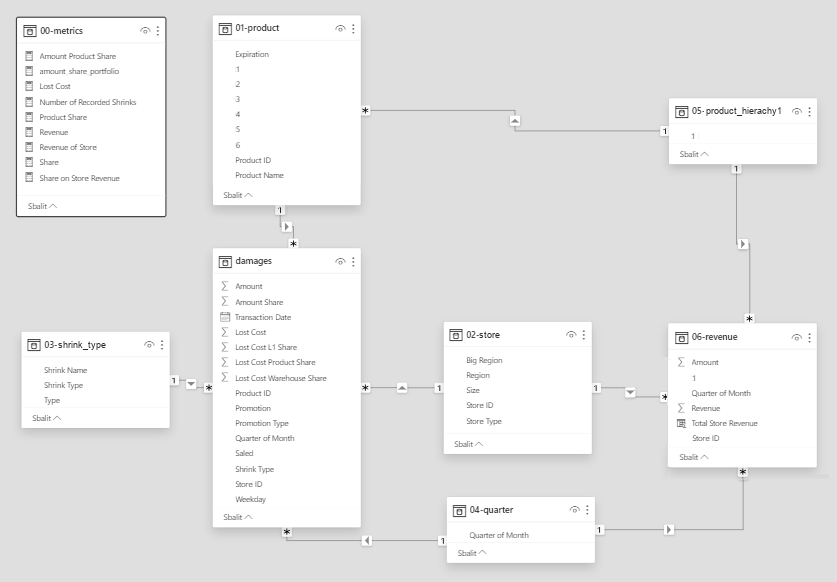
\includegraphics[width=\textwidth]{obrazky/PBI/datmodel.png}
    \caption{Datový model tabulek v Power BI reportu.}
    \label{obr:datmod}
\end{figure}

\subsection{Metriky}

Pro 

\subsection{Reporting}


\section{Výsledky}
\label{sec:vizualizace:vysl}
